\section{LGAD検出器}
\subsection{基本構造}
Low Gain Avalanche Diode (LGAD)検出器は、高い時間分解能が実現できる半導体検出器として期待されている。
以下の 図\ref{fg:LGAD} にLGAD検出器の構造を示す。
LGAD検出器は$p$型シリコン半導体をベースにしたシリコン半導体検出器で、アルミニウム電極の直下に$\rm{SiO_2}$の酸化膜がある。
LGAD検出器の$n$型半導体は、シリコンに不純物としてリンが、$p$型半導体は、不純物としてホウ素がドープしてある。
$pn$接合を作るために形成された表面の${n}^+$層の数 $\rm{\mu m}$下に、増幅層としてアクセプター濃度が高い濃度が高い$p^+$層をドープした構造になっている。
検出器に逆バイアス電圧をかけると、高濃度の$p^+$層によって、局所的に高電場領域を作り出すことができる。
検出器内で生成された電子正孔対が、高電場による電子雪崩によって増幅されることで、立ち上がりが速い信号を出力することができる。
また、増幅層の高電場によって電子正孔対が加速され、移動速度が大きくなるため、電極に誘起される信号の立ち上がりが速くなる。
そのため、増幅層のない一般的な半導体検出器と比べて、信号サイズが大きく、信号の立ち上がりを速くすることができるため、非常に高い時間分解能で荷電粒子を検出できる。


\begin{figure}[h]
    \centering
    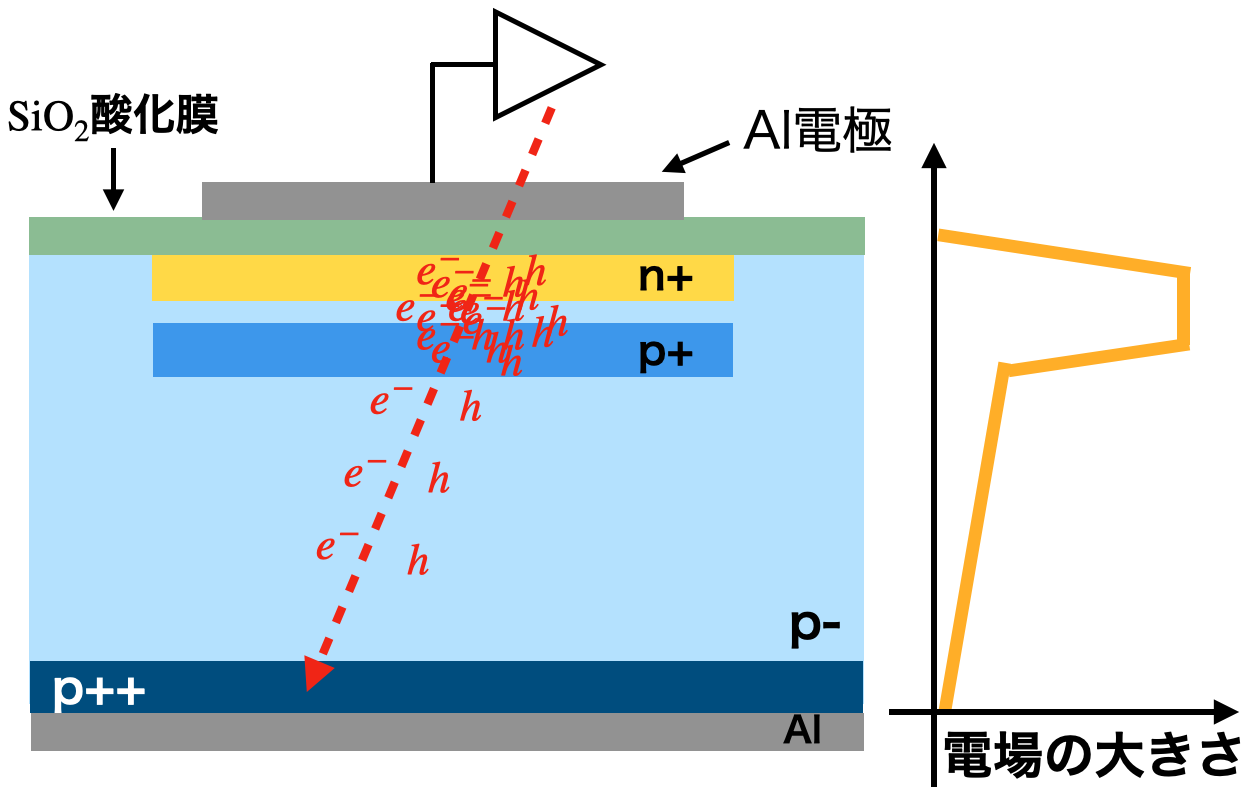
\includegraphics[width=8cm]{fig/ch1/LGAD.png}
    \caption[LGAD検出器の構造]{LGAD検出器の構造\\増幅層によって意図的に高電場を作り出し、電子雪崩によって電子正孔対が増幅される。立ち上がりの速い増幅された信号が出せるため、高い時間分解能が実現できる。}
    \label{fg:LGAD}
\end{figure}

\subsection{AD-LGAD検出器とDC-LGAD検出器}
従来のLGAD検出器は、電極ごとに増幅層を設置する 図\ref{fg:DC-LGAD} のようなDC-LGAD検出器であった。
DC-LGAD検出器では、電極の細密化によって、電極間に信号が確認できない不感領域ができてしまう問題があった。
そこで開発された 図\ref{fg:AC-LGAD} のAC-LGAD検出器は、増幅層を読み出し電極ごとに分割しないで一様に形成し、酸化膜を介して電極に誘起された信号を検出する。
\begin{figure}[h]
    \begin{minipage}[b]{0.5\linewidth}
        \centering
        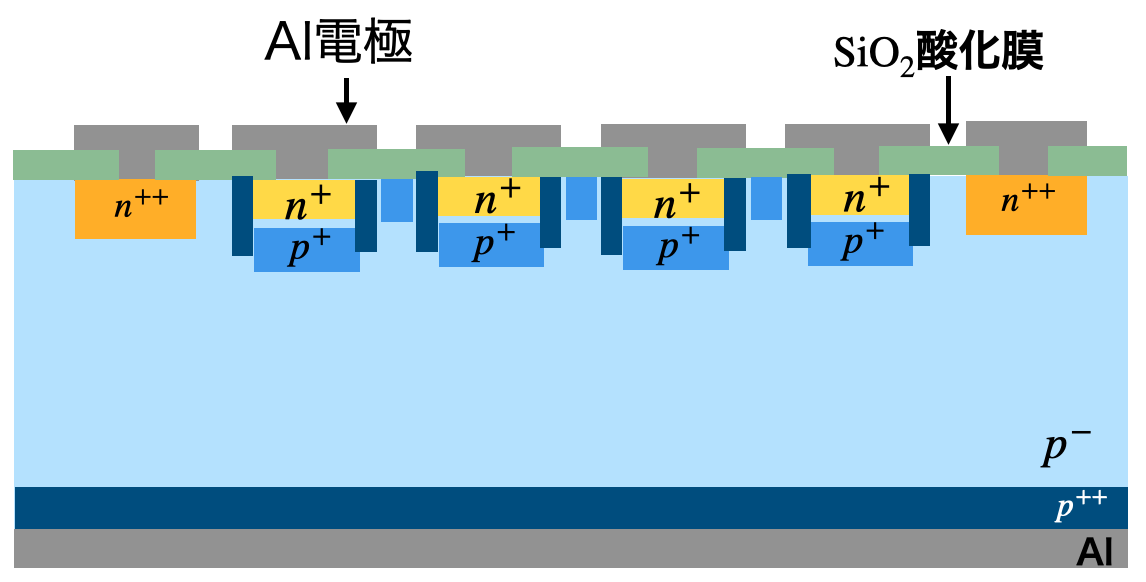
\includegraphics[width=7cm]{fig/ch3/DC-LGAD.png}
        \subcaption{DC-LGAD検出器}
        \label{fg:DC-LGAD}
    \end{minipage}
    \begin{minipage}[b]{0.5\linewidth}
        \centering
        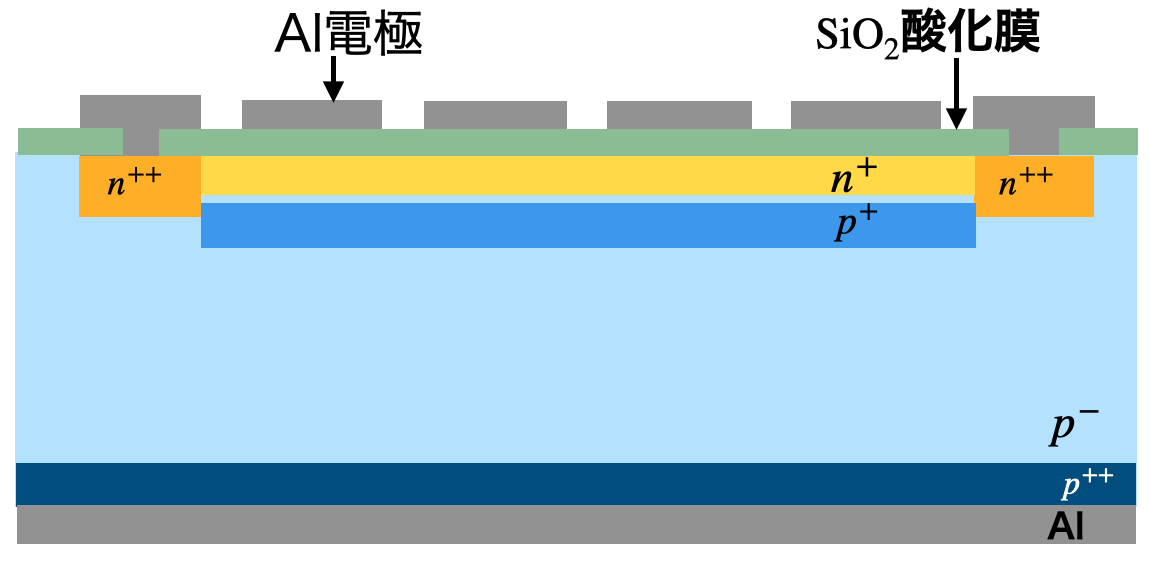
\includegraphics[width=7cm]{fig/ch3/AC-LGAD.png}
        \subcaption{AC-LGAD検出器}
        \label{fg:AC-LGAD}
    \end{minipage}
    \caption[DC-LGAD検出器とAC-LGAD検出器の構造]{DC-LGAD検出器とAC-LGAD検出器の構造\\DC-LGAD検出器は電極を細密化すると電極間に不感領域ができてしまう。\\AC-LGAD検出器は一様に増幅層を置くことで不感領域をなくすことができる。}
\end{figure}
増幅層を一様にしたことで、隣接チャンネルへの信号のクロストークが問題であったが、不純物濃度や酸化膜の厚さを最適化することで、
クロストークが抑制されたAC-LGAD検出器を開発されている\cite{kita2023development}。
本研究では、クロストークが最も少ないE600タイプのAC-LGAD検出器を使用する。

